%%%%%%%%%%%%%%%%%%%%%%%%%%%%%%%%%%%%%%%%%
% Lachaise Assignment
% LaTeX Template
% Version 1.0 (26/6/2018)
%
% This template originates from:
% http://www.LaTeXTemplates.com
%
% Authors:
% Marion Lachaise & François Févotte
% Vel (vel@LaTeXTemplates.com)
%
% License:
% CC BY-NC-SA 3.0 (http://creativecommons.org/licenses/by-nc-sa/3.0/)
% 
%%%%%%%%%%%%%%%%%%%%%%%%%%%%%%%%%%%%%%%%%

%----------------------------------------------------------------------------------------
%	PACKAGES AND OTHER DOCUMENT CONFIGURATIONS
%----------------------------------------------------------------------------------------

\documentclass{article}
\usepackage{graphicx}
\usepackage{amsmath}
\usepackage{bm}
\usepackage{steinmetz}
\graphicspath{{images/}}
\usepackage{float} 
\usepackage{mathtools}
\usepackage[american,RPvoltages]{circuiTikz}
\usepackage{tikz, tikz-cd}
\usepackage{pgfplots}
\usepackage{siunitx}
\usetikzlibrary{spy,shapes,arrows, arrows.meta, bending}
\pgfplotsset{width=10cm,compat=1.18}
\input{structure.tex} % Include the file specifying the document structure and custom commands
\renewcommand{\figurename}{Figura}
\usepackage{tcolorbox}
\usepackage{lipsum}
\tcbuselibrary{listings,theorems,skins,vignette,raster,breakable,magazine,poster,fitting,hooks}
\usepackage{svg}
%----------------------------------------------------------------------------------------
%	ASSIGNMENT INFORMATION
%----------------------------------------------------------------------------------------

\title{Método de superposición} % Title of the assignment
\author{Belmont Dubois} % Author name and email address

%----------------------------------------------------------------------------------------


\makeatletter
\pgfcircdeclarebipole{}{\ctikzvalof{bipoles/vsourcesin/height}}{sVpm}{\ctikzvalof{bipoles/vsourcesin/height}}{\ctikzvalof{bipoles/vsourcesin/width}}{
	
	\pgfsetlinewidth{\pgfkeysvalueof{/tikz/circuitikz/bipoles/thickness}\pgfstartlinewidth}
	\pgfpathellipse{\pgfpointorigin}{\pgfpoint{0}{\pgf@circ@res@up}}{\pgfpoint{\pgf@circ@res@left}{0}}
	\pgfusepath{draw}     
	\pgftext[bottom,rotate=90,y=\ctikzvalof{bipoles/vsourceam/margin}\pgf@circ@res@down]{\scriptsize$-$}
	\pgftext[top,rotate=90,y=\ctikzvalof{bipoles/vsourceam/margin}\pgf@circ@res@up]{\scriptsize$+$}
	
	\pgf@circ@res@up = .35\pgf@circ@res@up
	\pgfscope
	\pgftransformrotate{90}
	\pgfpathmoveto{\pgfpoint{-\pgf@circ@res@up}{0cm}}
	\pgfpathsine{\pgfpoint{.5\pgf@circ@res@up}{.4\pgf@circ@res@up}}
	\pgfpathcosine{\pgfpoint{.5\pgf@circ@res@up}{-.4\pgf@circ@res@up}}
	\pgfpathsine{\pgfpoint{.5\pgf@circ@res@up}{-.4\pgf@circ@res@up}}
	\pgfpathcosine{\pgfpoint{.5\pgf@circ@res@up}{.4\pgf@circ@res@up}}
	\pgfusepath{draw}
	\endpgfscope
}
\def\pgf@circ@sVpm@path#1{\pgf@circ@bipole@path{sVpm}{#1}}
\compattikzset{sinusoidal voltage source pm/.style = {\circuitikzbasekey, /tikz/to path=\pgf@circ@sVpm@path, \circuitikzbasekey/bipole/is voltage=true, \circuitikzbasekey/bipole/is voltageoutsideofsymbol=true, v=#1 }}
\compattikzset{sVpm/.style = {\comnpatname sinusoidal voltage source pm = #1}}

\pgfcircdeclarebipole{}{\ctikzvalof{bipoles/vsourcesin/height}}{sVpmh}{\ctikzvalof{bipoles/vsourcesin/height}}{\ctikzvalof{bipoles/vsourcesin/width}}{
	
	\pgfsetlinewidth{\pgfkeysvalueof{/tikz/circuitikz/bipoles/thickness}\pgfstartlinewidth}
	\pgfpathellipse{\pgfpointorigin}{\pgfpoint{0}{\pgf@circ@res@up}}{\pgfpoint{\pgf@circ@res@left}{0}}
	\pgfusepath{draw}     
	\pgftext[center,x=0.2\pgf@circ@res@down-\ctikzvalof{bipoles/vsourceam/margin}\pgf@circ@res@down]{\scriptsize$-$}
	\pgftext[top,rotate=90,y=\ctikzvalof{bipoles/vsourceam/margin}\pgf@circ@res@up]{\scriptsize$+$}
	
	\pgf@circ@res@up = .35\pgf@circ@res@up
	\pgfscope
	\pgftransformrotate{90}
	\pgfpathmoveto{\pgfpoint{-\pgf@circ@res@up}{0cm}}
	\pgfpathsine{\pgfpoint{.5\pgf@circ@res@up}{.4\pgf@circ@res@up}}
	\pgfpathcosine{\pgfpoint{.5\pgf@circ@res@up}{-.4\pgf@circ@res@up}}
	\pgfpathsine{\pgfpoint{.5\pgf@circ@res@up}{-.4\pgf@circ@res@up}}
	\pgfpathcosine{\pgfpoint{.5\pgf@circ@res@up}{.4\pgf@circ@res@up}}
	\pgfusepath{draw}
	\endpgfscope
}
\def\pgf@circ@sVpmh@path#1{\pgf@circ@bipole@path{sVpmh}{#1}}
\compattikzset{sinusoidal voltage source pmh/.style = {\circuitikzbasekey, /tikz/to path=\pgf@circ@sVpmh@path, \circuitikzbasekey/bipole/is voltage=true, \circuitikzbasekey/bipole/is voltageoutsideofsymbol=true, v=#1 }}
\compattikzset{sVpmh/.style = {\comnpatname sinusoidal voltage source pmh = #1}}
\makeatother

\begin{document}
	
	\maketitle % Print the title
	
	%----------------------------------------------------------------------------------------
	%	INTRODUCTION
	%----------------------------------------------------------------------------------------
	
	\section*{Análisis de circuito con superposición} % Unnumbered section
	Dado el circuito original de la figura \ref{fig:figura1} tenemos que encontrar los valores de $A$ e $i_a$ utilizando el teorema de superposición y de manera que satisfagan la ecuación

	
	
	\begin{figure}[H]
		\centering
			\begin{circuitikz}[american, cute inductors,scale=0.8]
				\draw (0,0) node[ground]{} to[V, l=$v_s$] (0, 8)
				to [short] ++(6,0)
				to [R, -*] ++(0,-4) coordinate (C1)
				to[short] ++(-3,0)
				to[D] ++(0,-4)
				to[R] ++(0,-3) node[ground]{};
				\draw (C1) to[short] ++(3,0)
				to[D] ++(0,-4)
				to[R] ++(0,-3) node[ground]{};
			\end{circuitikz}
		\caption{Circuito en el dominio del tiempo.}
		\label{fig:figura1}
	\end{figure}
	
	\noindent Como primer paso en la aplicación del teorema de superposición, desconectamos la fuente de corriente $i_a$ como se muestra en la figura 2. 
	\begin{figure}[H]
		\centering
		\begin{circuitikz}[american, cute inductors,scale=0.9]
			\draw (0,0) to[V, l=$v_s$] (0, 4)
						to[short, -o] (1,4)
						to[R, l=$R_1$, a=\SI{6}{\ohm}, f>_=$i_x$, o-o] (5,4)
						to[R, l2=$R_2$ and \SI{12}{\ohm},o-*] (5,0)
						to[short, -o] (1,0)
						to[short,o-] (0,0);
			\draw (5,4) to[cV, invert, l=$A\, i_x$, o-] (10,4)
						to[R, l2_=$R_3$ and \SI{12}{\ohm}, -*, v^=$v_{o1}$] (10,0)
						to[short] (4,0);
			\draw (10,4) to[short, *-o] (12,4);
			\draw (10,0) to[short, -o] (12,0);
			\draw[->]   (2.5,2.5) arc(110:-110:5mm) node[midway, left, font=\footnotesize] {$i_x$};
			\draw[->]   (7.5,2.5) arc(110:-110:5mm) node[midway, left, font=\footnotesize] {$i_2$};
		\end{circuitikz}
		\caption{Aplicando el teorema de superposición desconectando la fuente de corriente $i_a$}
		\label{fig:figura2}
	\end{figure}
	
	\noindent Aplicando la LTK sobre el lazo $i_x$ obtenemos:
	\begin{align}
		v_s - 6i_x - 12(i_x - i_2) = 0\nonumber\\
		v_s - 6i_x - 12i_x + 12i_2 = 0\nonumber\\
		18i_x - 12i_2 = v_s
	\end{align}
	
	\noindent Ahora aplicamos la LTK sobre el lazo $i_2$
	\begin{align}
		-12(i_2 - i_x) - Ai_x - 12i_2 = 0\nonumber\\
		-12i_2 + 12i_x - Ai_x - 12i_2 = 0\nonumber\\
		(12-A)i_x - 24i_2 = 0
	\end{align}

	\noindent Con lo cual tenemos el siguiente sistema de ecuaciones
	\begin{subequations}
		\begin{align}
			18 & i_x - 12i_2 = v_s\\
			(12-A)& i_x - 24i_2 = 0
		\end{align}	
	\end{subequations}
	
	\noindent Emplearemos el método de suma y resta para reducir nuestro sistema de ecuaciones en (3), para esto, multiplicamos la ecuación (3a) por (-2)
	
	\begin{align}
		-36i_x + 24i_2 &= -2v_s\nonumber\\
		(12-A)i_x - 24i_2 & = 0\nonumber \\
		\cline{1-2}
		(12-A-36)i_x  &= -2v_s\nonumber\\
		-(24+A)i_x &= -2v_s\nonumber\\
		i_x &= \frac{2v_s}{24+A} 
	\end{align}
	
	\noindent Como siguiente paso, despejamos $i_2$ de la ecuación (3b) y sustituimos el valor de (4)
	\begin{align}
		24i_2 &= (12-A)i_x\nonumber\\
		i_2 &= \frac{12-A}{24}i_x\nonumber\\
		i_2 &= \left( \frac{12-A}{24} \right)\left( \frac{2v_s}{24+A} \right)\nonumber\\
		i_2 &= \frac{(12-A)v_s}{12(24+A)} 
	\end{align}
	
	\noindent De esta manera, el voltaje $v_{o1}$ está dado por
	
	\begin{align}
		v_{o1} &= 12i_2 = \frac{12(12-A)v_s}{12(24+A)}\nonumber
	\end{align}
	
	\begin{tcolorbox}[colback=red!5!white,colframe=red!75!black,arc=0mm,boxrule=0mm,width=(\linewidth+0.5cm)]
		\begin{equation}
			v_{o1} = \frac{(12-A)v_s}{(24+A)}
		\end{equation}
	\end{tcolorbox}
	
	\noindent Con esto, hemos hallado el voltaje de salida $v_{o1}$ cuando la fuente de corriente $i_a$ no tiene efecto sobre el circuito. El siguiente paso es volver a activar la fuente de corriente $i_a$ y desconectar la fuente de tensión $v_s$ como se muestra en la figura 3.
	
	\begin{figure}[H]
		\centering
		\begin{circuitikz}[american, cute inductors,scale=0.9]
			\draw (0,0) to[R, l2=$R_1$ and \SI{6}{\ohm}] (0,4)
						to[short, f_=$i_x$, -*] (4,4)
						to[R, l2=$R_2$ and \SI{12}{\ohm}, -*] (4,0)
						to[short] (0,0);
			\draw (4,4) to[cV, invert, l=$Ai_x$, -*, i=$i_1$] (8,4)
						to[I, l=$i_a$, -*] (8,0)
						to[short] (4,0);
			\draw (8,4) to[short, i=$i_2$] (12,4)
						to[R, l2_=$R_3$ and \SI{12}{\ohm}, -*, v^=$v_{o2}$] (12,0)
						to[short] (8,0);
			\draw (12,4)to[short, *-o] (14,4);
			\draw (12,0)to[short, -o] (14,0);
			\draw[->]   (2,2.5) arc(110:-110:5mm) node[midway, left, font=\footnotesize] {$i_x$};
			\draw[->]   (6,2.5) arc(110:-110:5mm) node[midway, left, font=\footnotesize] {$i_1$};
			\draw[->]   (9.5,2.5) arc(110:-110:5mm) node[midway, left, font=\footnotesize] {$i_2$};
			\draw (8,4) node[above] {$v_{o2}$};
			%\draw (6,0) node[ground] {};
		\end{circuitikz}
		\caption{Aplicando el teorema de superposición desconectando la fuente de tensión  $v_s$}
		\label{fig:figura3}
	\end{figure}
	
	\noindent Empleamos la LTK sobre el lazo $i_x$
	\begin{align}
		-6i_x - 12(i_x - i_1) = 0\nonumber\\
		-6i_x - 12i_x + 12i_1 = 0\nonumber\\
		18i_x - 12i_1 = 0
	\end{align}
	
	\noindent Hay que tener en cuenta que hay una fuente de corriente sobre el lazo $i_2$ e $i_2$, teniendo así un súper lazo
	\begin{align}
		-12(i_1 - i_x) - Ai_x - 12i_2 = 0\nonumber\\
		-12i_1 + 12i_x - Ai_x - 12i_2 = 0\nonumber\\
		(12-A)i_x - 12i_1 - 12i_2 = 0
	\end{align}
	
	\noindent Al emplear la Ley de Corrientes de Kirchhoff (LCK) sobre el nodo $v_{o2}$ obtenemos
	\begin{align}
		i_1 = i_a + i_2
	\end{align}
	
	\noindent Al sustituir la ecuación (9) en (8) obtenemos
	\begin{align}
		(12-A)i_x - 12(i_a + i_2) - 12i_2 &= 0\nonumber\\
		(12-A)i_x - 12i_a - 12i_2 - 12i_2 &= 0\nonumber\\
		(12-A)i_x - 12i_a - 24i_2 &= 0\nonumber\\
		(12-A)i_x - 24i_2 &= 12i_a
	\end{align}
	
	\noindent Sustituimos también la ecuación (9) en (7)
	\begin{align}
		18i_x - 12(i_a + i_2) &= 0\nonumber\\
		18i_x - 12i_a - 12i_2 &= 0\nonumber\\
		18i_x - 12i_2 &= 12i_a
	\end{align}
	
	\noindent De las ecuaciones (10) y (11) conseguimos nuestro nuevo sistema de ecuaciones
	\begin{subequations}
		\begin{align}
			(12-A)i_x - 24i_2 &= 12i_a\\
			18i_x - 12i_2 &= 12i_a
		\end{align}	
	\end{subequations}
	
	\noindent Volvemos a emplear el método de suma y resta para encontrar el valor de $i_x$ multiplicando la ecuación (12b) por (-2)
	\begin{align}
		(12-A)i_x - 24i_2 &= 12i_a\nonumber\\
		-36i_x + 24i_2 &= -24i_a\nonumber \\
		\cline{1-2}
		(12-A-36)i_x  &= -12i_a\nonumber\\
		-(24+A)i_x &= -12i_a\nonumber\\
		i_x &= \frac{12i_a}{24+A} 
	\end{align}
	
	\noindent Despejamos $i_2$ de la ecuación (12a)
	\begin{align}
		24i_2 &= (12-A)i_x - 12i_a\nonumber\\
		i_2 &= \frac{(12-A)i_x}{24} - \frac{12i_a}{24}
	\end{align}
	
	\noindent Simplificamos y sustituimos el valor de $i_x$ de la ecuación (13) en (14)
	\begin{align}
		i_2 &= \left( \frac{12-A}{24} \right) \left( \frac{12i_a}{24+A} \right) - \frac{12i_a}{24}\nonumber\\
		 &= \left( \frac{12-A}{2} \right) \left( \frac{i_a}{24+A} \right) - \frac{i_a}{2}\nonumber\\
		&= \frac{(12-A)i_a}{2(24+A)} - \frac{i_a}{2}\nonumber\\
		&= \frac{(12-A)i_a - (24 + A)i_a}{2(24+A)} = \frac{-12i_a - 2Ai_a}{2(24+A)}\nonumber
	\end{align}
	
	\noindent Es decir
	\begin{align}
		i_2 = -\frac{(6 + A)i_a}{24+A}
	\end{align}
	
	\noindent El voltaje de salida está dado por:
	\begin{align}
		v_{o2} = 12i_2 = -\frac{12(6+A)i_a}{24+A}\nonumber
	\end{align}
	
	\begin{tcolorbox}[colback=red!5!white,colframe=red!75!black,arc=0mm,boxrule=0mm,width=(\linewidth+0.5cm)]
		\begin{equation}
			v_{o2} = -\frac{12(6+A)i_a}{24+A}
		\end{equation}
	\end{tcolorbox}
	
	\noindent Juntando las ecuaciones (6) y (16) obtenemos el voltaje de salida completo del circuito de la figura 1:
	\begin{tcolorbox}[colback=red!5!white,colframe=red!75!black,arc=0mm,boxrule=0mm,width=(\linewidth+0.5cm)]
		\begin{equation}
			v_{o} = v_{o1} + v_{o2} = \frac{(12-A)v_s}{(24+A)} -\frac{12(6+A)i_a}{24+A}
		\end{equation}
	\end{tcolorbox}
	
	\noindent Sin embargo debemos hacer que nuesra voltaje de salida sea igual a $v_o = 2v_s + 9$, por lo tanto
	\begin{align*}
		v_{o} = \underbrace{\frac{(12-A)}{(24+A)}}_{=2} v_s \underbrace{-\frac{12(6+A)i_a}{24+A}}_{=9} 
	\end{align*}
	
	\begin{align*}
		\frac{(12-A)}{(24+A)} = 2\\
		12-A = 2(24 + A)\\
		12-A = 48 + 2A\\
		3A = 12-48\\
		A = -\frac{36}{3}\\
	\end{align*}
	
	\begin{tcolorbox}[colback=red!5!white,colframe=red!75!black,arc=0mm,boxrule=0mm,width=(\linewidth+0.5cm)]
		\begin{equation}
			A = -12
		\end{equation}
	\end{tcolorbox}
	
	\noindent Y
	\begin{align*}
		-\frac{12(6+A)i_a}{24+A}=9\\
		-12(6+A)i_a = 9(24 + A)\\
		-12(6+A)i_a = 216 + 9A\\
		i_a = -\frac{216 + 9A}{12(6+A)}  
	\end{align*}
	
	\begin{tcolorbox}[colback=red!5!white,colframe=red!75!black,arc=0mm,boxrule=0mm,width=(\linewidth+0.5cm)]
		\begin{equation}
			i_a = \SI{1.5}{\ampere}
		\end{equation}
	\end{tcolorbox}
	
	El signo negativo en el valor de $A$ en la ecuación 18 indica que en realidad la polaridad debería estar invertida, si realizas la simulación en algún software como Multisim, por ejemplo, tienes dos opciones, expresar la cantidad negativa con la misma polaridad que se presenta en la figura 1 o expresar la cantidad positiva pero invirtiendo la polaridad de la fuente de tensión dependiente de corriente.
	
	 %trim={<left> <lower> <right> <upper>}
	\begin{figure}[H]
		\centering
		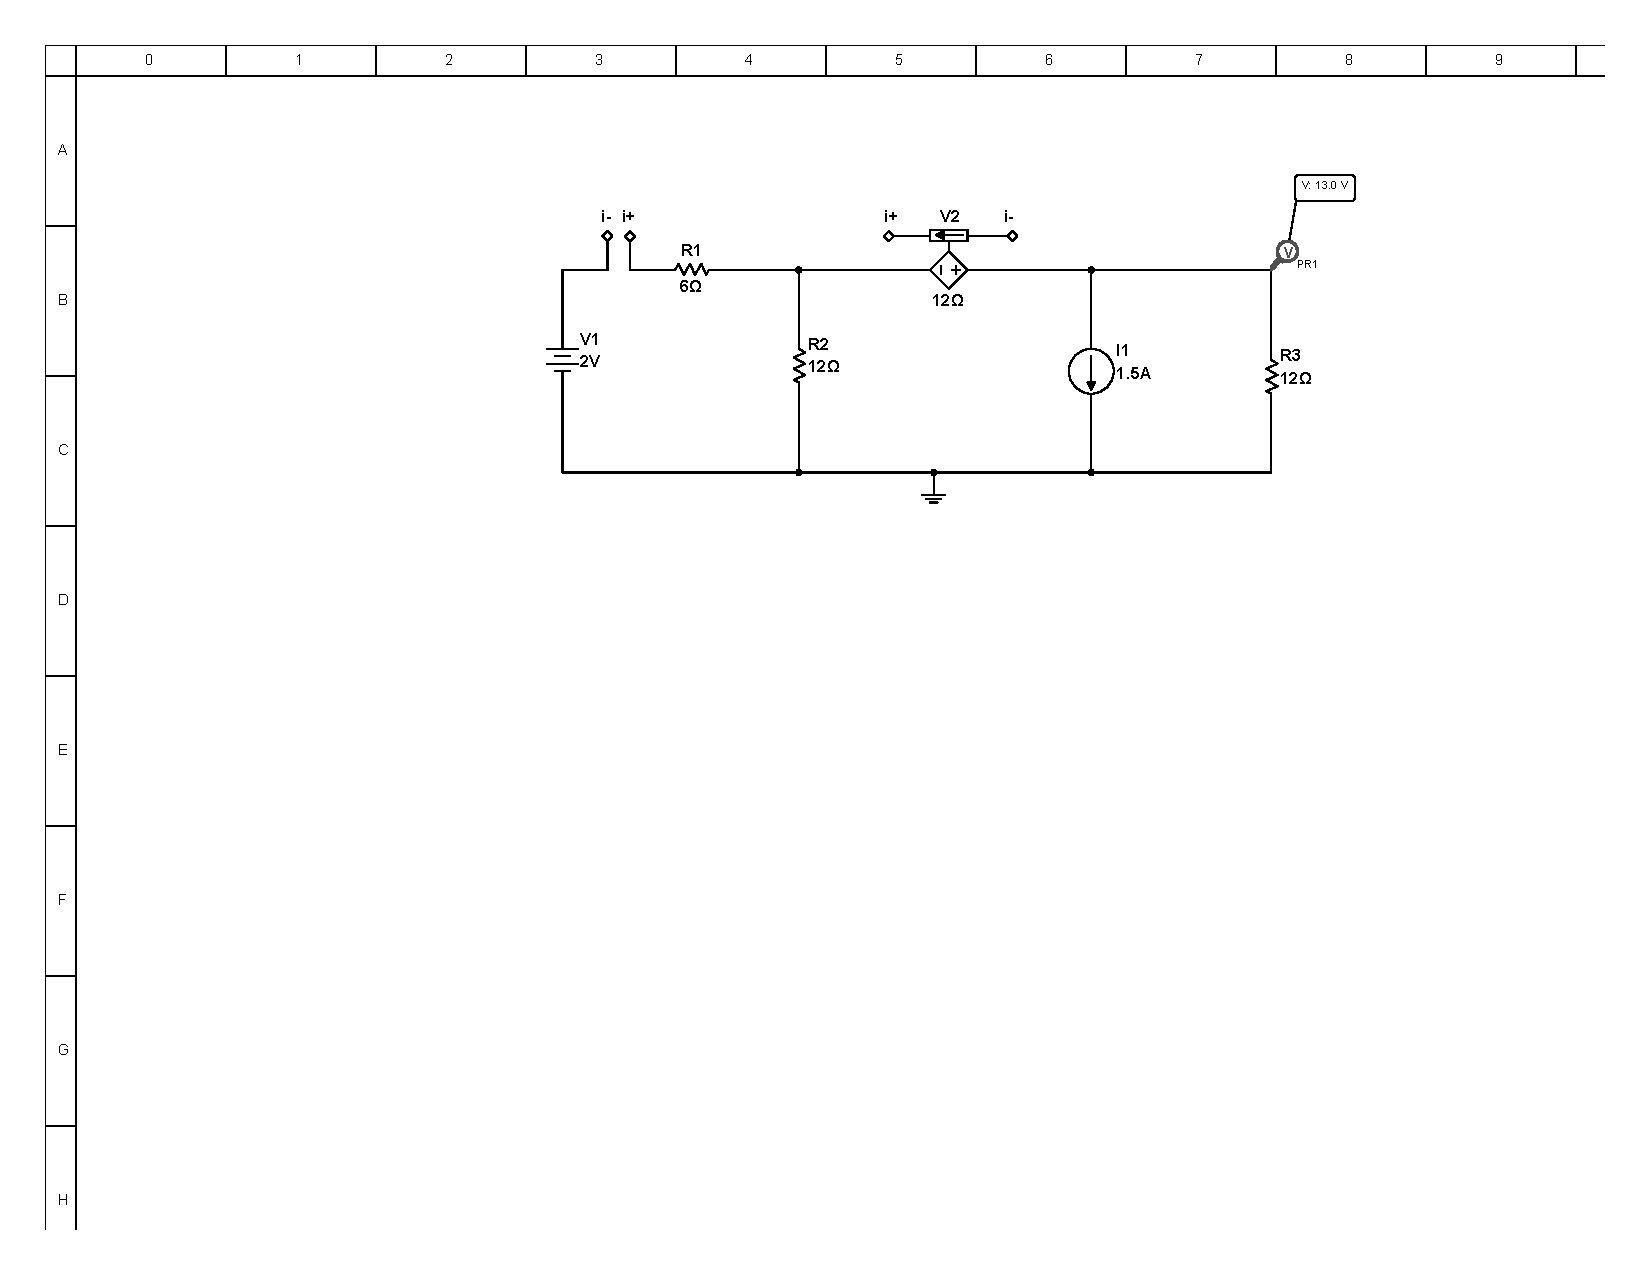
\includegraphics[scale=1,trim={9cm 12.5cm 5cm 2.5cm},clip]{cto}
		\caption{Simulación del circuito}
		\label{fig:figura4}
	\end{figure}
		
	
	
	%\begin{circuitikz}[scale=0.8]
	%	\draw (0,0) to[R, l=$R_1$, o-] ++(2,0) %++(x,y) recuerda la última corrdenada, en este caso, se mueve dos unidades a la derecha
	%				to[R, l=$R_2$] ++(2,0)
	%				to[R, l=$R_3$] ++(2,0) coordinate(a);
	%	\draw 		[dashed] (a) -- ++(1,0) coordinate(b);
	%	\draw (b)	to[R, l=$R_n$, -o] ++(2,0) coordinate(c);
	%	\draw (10,0) node[right] {$ \Rightarrow$};
	%	\draw (11,0) to[R, l=$R_{eq}$, o-o] ++(2,0);
	%	%\draw (8,4) node[above] {$v_{o2}$};
	%\end{circuitikz}
	
	\begin{circuitikz}[color=black]
		\draw (8,0) node[npn](Q1){};
		\draw (Q1.E) to[R, l2^=$R_E$ and \SI{5}{k\ohm}] ++(0,-3) node[vee](VEE){$V_{EE}=\SI{-10}{V}$};
		\draw (Q1.E) to[short, *-] ++(2,0) to[C=$C_1$] ++(0,-2.5) node[ground]{};
		\draw (Q1.C) to[R, l2^=$R_E$ and \SI{5}{k\ohm}] ++(0,3) node[vcc](VCC){$V_{CC}=\SI{10}{V}$};
		\draw (Q1.C) to[short, *-] ++(5,0) coordinate(input);
		\draw (Q1.B) to[short] ++(-1,0) coordinate(in) to[R] ++(0,-3) node[ground]{};
		\draw (in) to[C, *-o] ++(-3,0) node[left]{$v_1$};
		\draw (input) node[npn, right](Q2){};
		\draw (Q2.E) to[R] ++(0,-3);
	\end{circuitikz}
\end{document}


